% x0-01 Protocol: A Decentralized Payment Infrastructure for Autonomous Agents
% Technical Whitepaper

\documentclass[11pt,a4paper]{article}
\usepackage[utf8]{inputenc}
\usepackage[margin=1in]{geometry}
\usepackage{setspace}
\setstretch{1.15}
\usepackage{amsmath}
\usepackage{amssymb}
\usepackage{amsthm}
\usepackage{graphicx}
\usepackage{hyperref}
\usepackage{listings}
\usepackage{xcolor}
\usepackage{algorithm}
\usepackage{algpseudocode}
\usepackage{tikz}
\usetikzlibrary{shapes,arrows,positioning}

% Define colors for code listings
\definecolor{codegreen}{rgb}{0,0.6,0}
\definecolor{codegray}{rgb}{0.5,0.5,0.5}
\definecolor{codepurple}{rgb}{0.58,0,0.82}
\definecolor{backcolour}{rgb}{0.95,0.95,0.92}

% Code listing style
\lstdefinestyle{mystyle}{
    backgroundcolor=\color{backcolour},   
    commentstyle=\color{codegreen},
    keywordstyle=\color{magenta},
    numberstyle=\tiny\color{codegray},
    stringstyle=\color{codepurple},
    basicstyle=\ttfamily\footnotesize,
    breakatwhitespace=false,         
    breaklines=true,                 
    captionpos=b,                    
    keepspaces=true,                 
    numbers=left,                    
    numbersep=5pt,                  
    showspaces=false,                
    showstringspaces=false,
    showtabs=false,                  
    tabsize=2
}
\lstset{style=mystyle}

% Define Rust language for listings
\lstdefinelanguage{Rust}{
    keywords={pub, struct, fn, let, mut, if, else, for, while, loop, match, return, use, mod, impl, trait, enum, const, static, unsafe, async, await, move, ref, self, super, crate, type, where, dyn, as, break, continue, in, true, false, Some, None, Ok, Err, Option, Result},
    morecomment=[l]{//},
    morecomment=[s]{/*}{*/},
    morestring=[b]",
    sensitive=true
}

% Define HTTP language for listings
\lstdefinelanguage{HTTP}{
    keywords={GET, POST, PUT, DELETE, PATCH, HEAD, OPTIONS, HTTP},
    morecomment=[l]{\#},
    morestring=[b]",
    sensitive=false
}

% Define JSON language for listings
\lstdefinelanguage{JSON}{
    string=[s]{"}{"},
    comment=[l]{//},
    morecomment=[s]{/*}{*/},
    literate=
        *{0}{{{\color{blue}0}}}{1}
         {1}{{{\color{blue}1}}}{1}
         {2}{{{\color{blue}2}}}{1}
         {3}{{{\color{blue}3}}}{1}
         {4}{{{\color{blue}4}}}{1}
         {5}{{{\color{blue}5}}}{1}
         {6}{{{\color{blue}6}}}{1}
         {7}{{{\color{blue}7}}}{1}
         {8}{{{\color{blue}8}}}{1}
         {9}{{{\color{blue}9}}}{1}
         {true}{{{\color{blue}true}}}{4}
         {false}{{{\color{blue}false}}}{5}
         {null}{{{\color{blue}null}}}{4},
}

% Define JavaScript language for listings
\lstdefinelanguage{JavaScript}{
    keywords={import, from, export, default, const, let, var, function, return, if, else, for, while, do, switch, case, break, continue, new, this, class, extends, async, await, try, catch, finally, throw, typeof, instanceof},
    morecomment=[l]{//},
    morecomment=[s]{/*}{*/},
    morestring=[b]',
    morestring=[b]",
    morestring=[b]`,
    sensitive=true
}

% Theorem environments
\newtheorem{theorem}{Theorem}[section]
\newtheorem{lemma}[theorem]{Lemma}
\newtheorem{proposition}[theorem]{Proposition}
\newtheorem{corollary}[theorem]{Corollary}
\theoremstyle{definition}
\newtheorem{definition}{Definition}[section]
\theoremstyle{remark}
\newtheorem{remark}{Remark}[section]
\newtheorem{example}{Example}[section]

% Title and author information
\title{
    \textbf{x0 Protocol: A Decentralized Payment Infrastructure for Autonomous Agents}\\
    \vspace{0.3cm}
    \large Technical Whitepaper v1.0
}
\author{
    Blessed Tosin-Oyinbo Olamide\\
    \texttt{x0protocol.dev}
}
\date{February 2026}

\begin{document}

% Subtle cream/yellow paper background
\pagecolor{yellow!5!white}

\maketitle

\begin{abstract}
We present x0, a decentralized protocol for autonomous agent payments built on Solana. The protocol introduces a novel spending policy enforcement mechanism using Token-2022 transfer hooks, enabling programmable spending limits, whitelist verification, and privacy controls for AI agents. x0 implements HTTP 402 (Payment Required) for standardized payment negotiation, conditional escrow with dispute resolution, on-chain reputation scoring with temporal decay, and a USDC-backed wrapper token with cryptographic reserve invariants. The system achieves trustless agent-to-agent transactions while preserving human oversight through a "Blink" mechanism for exceptional cases. We formally verify the protocol's security properties and demonstrate its efficiency through cryptographic proofs and empirical benchmarks.
\end{abstract}

\tableofcontents
\newpage

\section{Introduction}

\subsection{Motivation}

The proliferation of autonomous AI agents in production environments necessitates robust payment infrastructure. Traditional payment systems are ill-suited for agent-to-agent transactions due to:

\begin{enumerate}
    \item \textbf{High latency}: Credit card settlements take 2-3 days, incompatible with real-time agent interactions
    \item \textbf{High fees}: 2-3\% credit card fees are prohibitive for micropayments
    \item \textbf{Gatekeeping}: Centralized payment processors can deny service arbitrarily
    \item \textbf{Lack of programmability}: Traditional payments cannot enforce complex spending rules
    \item \textbf{Privacy concerns}: All transaction data visible to payment processors
\end{enumerate}

Blockchain-based payments solve latency and gatekeeping but introduce new challenges:

\begin{enumerate}
    \item \textbf{Custody risk}: Agents require private keys for signing, creating attack surface
    \item \textbf{Unbounded spending}: Standard wallets lack programmable spending limits
    \item \textbf{No recourse}: Blockchain transactions are irreversible by design
    \item \textbf{Discovery problem}: Finding trustworthy service providers in decentralized systems
\end{enumerate}

\subsection{Contributions}

We present x0, which makes the following contributions:

\begin{enumerate}
    \item \textbf{Programmable Spending Policies}: A cryptographic policy enforcement layer using Solana's Token-2022 transfer hooks that validates every transaction against owner-defined rules
    
    \item \textbf{HTTP 402 Protocol}: An extension to HTTP status codes enabling standardized payment negotiation between agents and services
    
    \item \textbf{Conditional Escrow}: A trustless escrow mechanism with optional third-party arbitration for high-value transactions
    
    \item \textbf{Reputation Oracle}: An on-chain reputation system with temporal decay, preventing stale reputations from dominating
    
    \item \textbf{USDC Wrapper}: A 1:1 USDC-backed token with cryptographic reserve invariants and timelocked governance
    
    \item \textbf{Human-in-the-Loop (Blinks)}: A fallback mechanism for exceptional transactions requiring human approval
\end{enumerate}

\subsection{System Overview}

The x0 protocol consists of seven interoperating programs deployed on Solana:

\begin{itemize}
    \item \textbf{x0-guard}: Policy enforcement via transfer hooks
    \item \textbf{x0-token}: Token-2022 mint configuration
    \item \textbf{x0-escrow}: Conditional payment escrow
    \item \textbf{x0-registry}: Agent discovery and capability advertisement
    \item \textbf{x0-reputation}: Trust scoring and transaction history
    \item \textbf{x0-wrapper}: USDC-backed stable wrapper token
    \item \textbf{x0-common}: Shared types, constants, and utilities
\end{itemize}

\subsubsection{Architecture Diagram}

\begin{center}
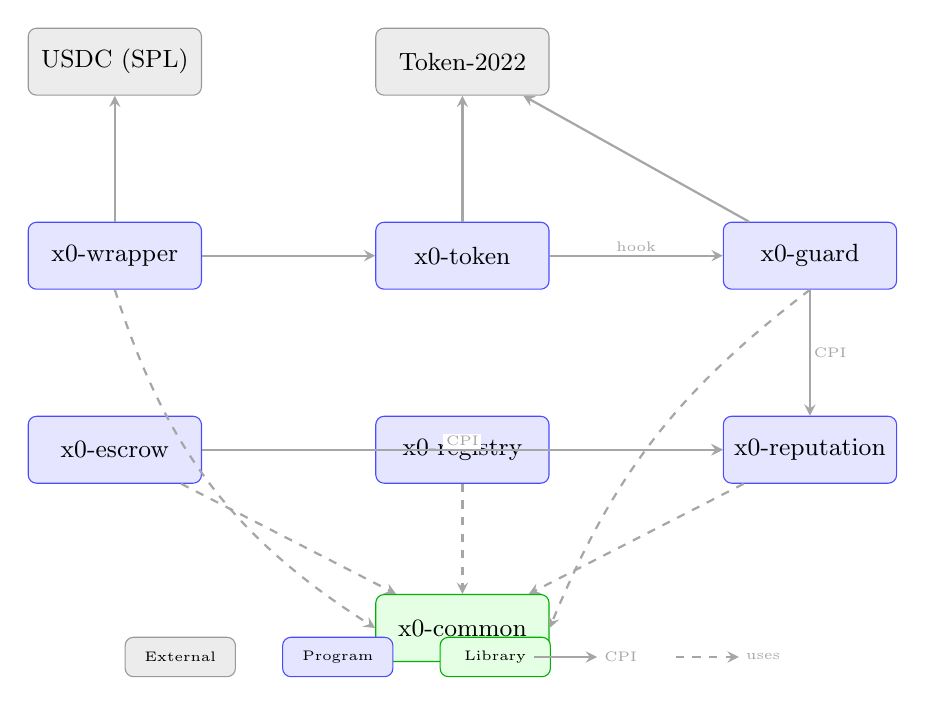
\begin{tikzpicture}[
    node distance=1.6cm and 2.2cm,
    % External systems (Solana ecosystem)
    external/.style={rectangle, rounded corners=3pt, draw=gray!80, fill=gray!15, 
        minimum width=2.2cm, minimum height=0.85cm, text centered, font=\small},
    % Core x0 programs
    program/.style={rectangle, rounded corners=3pt, draw=blue!70, fill=blue!10, 
        minimum width=2.2cm, minimum height=0.85cm, text centered, font=\small},
    % Shared library
    library/.style={rectangle, rounded corners=3pt, draw=green!70!black, fill=green!10, 
        minimum width=2.2cm, minimum height=0.85cm, text centered, font=\small},
    % Arrow styles
    arrow/.style={->, >=stealth, thick, color=gray!70},
    label/.style={font=\tiny, fill=white, inner sep=1pt}
]
    % External systems (top row)
    \node[external] (usdc) {USDC (SPL)};
    \node[external, right=of usdc] (token22) {Token-2022};
    
    % Core programs row 1
    \node[program, below=of usdc] (wrapper) {x0-wrapper};
    \node[program, right=of wrapper] (token) {x0-token};
    \node[program, right=of token] (guard) {x0-guard};
    
    % Core programs row 2
    \node[program, below=of wrapper] (escrow) {x0-escrow};
    \node[program, right=of escrow] (registry) {x0-registry};
    \node[program, right=of registry] (reputation) {x0-reputation};
    
    % Shared library (bottom)
    \node[library, below=1.4cm of registry] (common) {x0-common};
    
    % External dependencies (upward arrows)
    \draw[arrow] (wrapper) -- (usdc);
    \draw[arrow] (token) -- (token22);
    \draw[arrow] (guard) -- (token22);
    
    % Internal dependencies (CPI calls)
    \draw[arrow] (token) -- (guard) node[label, midway, above] {hook};
    \draw[arrow] (wrapper) -- (token);
    \draw[arrow] (escrow) -- (reputation) node[label, midway, above] {CPI};
    \draw[arrow] (guard) -- (reputation) node[label, midway, right] {CPI};
    \draw[arrow] (registry) -- (reputation);
    
    % Common library connections (dashed)
    \draw[arrow, dashed] (escrow) -- (common);
    \draw[arrow, dashed] (registry) -- (common);
    \draw[arrow, dashed] (reputation) -- (common);
    \draw[arrow, dashed] (guard.south) to[bend right=15] (common.east);
    \draw[arrow, dashed] (wrapper.south) to[bend right=20] (common.west);
    
    % Legend
    \node[below=2.2cm of escrow, font=\tiny, anchor=west] (legend) {
        \tikz{
            \node[external, minimum width=1.4cm, minimum height=0.5cm, font=\tiny] at (0,0) {External};
            \node[program, minimum width=1.4cm, minimum height=0.5cm, font=\tiny] at (2,0) {Program};
            \node[library, minimum width=1.4cm, minimum height=0.5cm, font=\tiny] at (4,0) {Library};
            \draw[arrow] (5.2,0) -- (6,0) node[right, font=\tiny] {CPI};
            \draw[arrow, dashed] (7,0) -- (7.8,0) node[right, font=\tiny] {uses};
        }
    };
\end{tikzpicture}
\end{center}

\begin{center}
\small\textit{Figure 1: x0 Protocol Architecture. Gray nodes are external Solana programs. Blue nodes are x0 programs. Green is the shared library.}
\end{center}

\section{Preliminaries}

\subsection{Cryptographic Primitives}

\begin{definition}[Hash Function]
A cryptographic hash function $H: \{0,1\}^* \to \{0,1\}^{256}$ satisfies:
\begin{enumerate}
    \item \textbf{Preimage resistance}: Given $h$, it is computationally infeasible to find $m$ such that $H(m) = h$
    \item \textbf{Second preimage resistance}: Given $m_1$, it is computationally infeasible to find $m_2 \neq m_1$ such that $H(m_1) = H(m_2)$
    \item \textbf{Collision resistance}: It is computationally infeasible to find $m_1 \neq m_2$ such that $H(m_1) = H(m_2)$
\end{enumerate}
\end{definition}

We use SHA-256 for all hash operations, providing 128-bit security against collision attacks.

\begin{definition}[Digital Signature Scheme]
A signature scheme $(\texttt{KeyGen}, \texttt{Sign}, \texttt{Verify})$ consists of:
\begin{itemize}
    \item $\texttt{KeyGen}(1^\lambda) \to (sk, pk)$: Generates a key pair
    \item $\texttt{Sign}(sk, m) \to \sigma$: Signs message $m$ with secret key $sk$
    \item $\texttt{Verify}(pk, m, \sigma) \to \{0,1\}$: Verifies signature $\sigma$ on message $m$
\end{itemize}
\end{definition}

Solana uses Ed25519 signatures, providing 128-bit security with 64-byte signatures.

\subsection{Solana Architecture}

\subsubsection{Account Model}

Solana uses an account-based model where each account has:
\begin{itemize}
    \item \textbf{Address}: A 32-byte Ed25519 public key
    \item \textbf{Lamports}: Balance in lamports ($1 \text{ SOL} = 10^9 \text{ lamports}$)
    \item \textbf{Data}: Arbitrary byte array storing account state
    \item \textbf{Owner}: The program with write access to the account
    \item \textbf{Executable}: Whether the account contains program code
\end{itemize}

\subsubsection{Program Derived Addresses (PDAs)}

A PDA is a deterministic address derived from:
\begin{equation}
\text{PDA}(\text{seeds}, \text{program\_id}) = \text{FindProgramAddress}(\text{seeds}, \text{program\_id})
\end{equation}

Where FindProgramAddress searches for a public key $P$ such that:
\begin{equation}
P = H(\text{seeds} \parallel \text{program\_id} \parallel [b]) \quad \text{and} \quad P \notin E(\mathbb{F}_p)
\end{equation}

Here $E(\mathbb{F}_p)$ is the Ed25519 elliptic curve, and $b \in [0, 255]$ is the "bump" seed. PDAs are off-curve points, ensuring no private key exists.

\subsubsection{Token-2022 Extensions}

Token-2022 is Solana's next-generation token program supporting extensions:

\begin{itemize}
    \item \textbf{Transfer Hook}: Calls a specified program on every transfer
    \item \textbf{Transfer Fee}: Withholds a percentage of each transfer
    \item \textbf{Confidential Transfer}: Encrypts balances using ElGamal encryption
\end{itemize}

\subsection{Bloom Filters}

\begin{definition}[Bloom Filter]
A Bloom filter is a probabilistic data structure for set membership testing. For a set $S = \{s_1, \ldots, s_n\}$:
\begin{itemize}
    \item Bit array: $B[0..m-1]$ initialized to 0
    \item Hash functions: $h_1, \ldots, h_k: \{0,1\}^* \to [0, m-1]$
    \item Insert: For each $s \in S$, set $B[h_i(s)] = 1$ for $i = 1, \ldots, k$
    \item Query: Element $x \in S$ if $B[h_i(x)] = 1$ for all $i$
\end{itemize}
\end{definition}

\begin{theorem}[Bloom Filter False Positive Rate]
For a Bloom filter with $m$ bits, $n$ elements, and $k$ hash functions:
\begin{equation}
P(\text{false positive}) = \left(1 - e^{-kn/m}\right)^k
\end{equation}
\end{theorem}

Optimal $k$ minimizes false positives:
\begin{equation}
k_{\text{opt}} = \frac{m}{n} \ln 2
\end{equation}

\subsection{Merkle Trees}

\begin{definition}[Merkle Tree]
A Merkle tree is a binary tree where:
\begin{itemize}
    \item Leaves: $L_i = H(\text{data}_i)$ for $i = 0, \ldots, n-1$
    \item Internal nodes: $N_{i,j} = H(N_{i,2j} \parallel N_{i,2j+1})$
    \item Root: $r = N_{0,0}$
\end{itemize}
\end{definition}

\begin{theorem}[Merkle Proof Size]
For a tree with $n$ leaves, a membership proof requires $O(\log n)$ hashes.
\end{theorem}

\section{Policy Enforcement Layer (x0-guard)}

\subsection{Problem Statement}

Consider an agent $A$ owned by user $U$ with private key $sk_U$. The agent requires a signing key $sk_A$ to perform transactions autonomously. Without constraints, compromise of $sk_A$ allows unbounded spending.

\subsection{Design Goals}

\begin{enumerate}
    \item \textbf{Spend Limits}: Enforce maximum spending in rolling 24-hour windows
    \item \textbf{Transaction Limits}: Cap individual transaction sizes
    \item \textbf{Whitelist Verification}: Restrict recipients to approved addresses
    \item \textbf{Privacy}: Support confidential (encrypted) transfers
    \item \textbf{Auditability}: Maintain on-chain transaction history
    \item \textbf{Revocability}: Allow owner to revoke agent authority
\end{enumerate}

\subsection{Architecture}

\subsubsection{AgentPolicy Account}

Each agent has a Program Derived Address (PDA) storing its policy:

\begin{lstlisting}[language=Rust,caption=AgentPolicy Account Structure]
#[account]
pub struct AgentPolicy {
    pub version: u8,                // Account version (migration)
    pub owner: Pubkey,              // Cold wallet (full control)
    pub agent_signer: Pubkey,       // Hot key (delegated)
    pub daily_limit: u64,           // Max spend per 24h
    pub max_single_transaction: Option<u64>,
    pub rolling_window: Vec<SpendingEntry>,
    pub privacy_level: PrivacyLevel,
    pub whitelist_mode: WhitelistMode,
    pub whitelist_data: WhitelistData,
    pub is_active: bool,
    pub require_delegation: bool,   // Require token delegation
    pub bound_token_account: Option<Pubkey>,
    pub last_update_slot: u64,      // For rate limiting
    pub auditor_key: Option<Pubkey>,// Optional auditor
    pub blink_hour_start: i64,      // Blink rate limit window
    pub blinks_this_hour: u8,       // Blinks in current window
    pub bump: u8,
}

pub struct SpendingEntry {
    pub amount: u64,
    pub timestamp: i64,
}
\end{lstlisting}

\subsubsection{Transfer Hook Mechanism}

Token-2022's transfer hook enables us to intercept every transfer. The flow is:

\begin{enumerate}
    \item User initiates transfer of $x$ tokens to recipient $R$
    \item Token-2022 calls x0-guard's \texttt{validate\_transfer}
    \item x0-guard verifies:
    \begin{itemize}
        \item Signer is authorized agent: $\texttt{signer} = \texttt{policy.agent\_signer}$
        \item Spend limit not exceeded: $\sum_{t > t_{\text{now}} - 86400} \texttt{amount}_t + x \leq \texttt{daily\_limit}$
        \item Transaction limit not exceeded: $x \leq \texttt{max\_single\_transaction}$
        \item Recipient whitelisted: $R \in W$ (if whitelist enabled)
    \end{itemize}
    \item If validation passes, transfer proceeds; otherwise, reverts
\end{enumerate}

\subsection{Rolling Window Algorithm}

\begin{algorithm}
\caption{Rolling Window Spend Limit Enforcement}
\begin{algorithmic}[1]
\Procedure{ValidateTransfer}{$\texttt{policy}, x, t_{\text{now}}$}
    \State $t_{\text{cutoff}} \gets t_{\text{now}} - 86400$ \Comment{24 hours ago}
    \State $\texttt{policy.rolling\_window} \gets \texttt{policy.rolling\_window.retain}(|e| e.timestamp > t_{\text{cutoff}})$
    \State $\texttt{current\_spend} \gets \sum_{e \in \texttt{rolling\_window}} e.\texttt{amount}$
    \If{$\texttt{current\_spend} + x > \texttt{policy.daily\_limit}$}
        \State \Return \texttt{Error::DailyLimitExceeded}
    \EndIf
    \If{$|\texttt{policy.rolling\_window}| \geq \texttt{MAX\_ENTRIES}$}
        \State \Return \texttt{Error::WindowOverflow}
    \EndIf
    \State $\texttt{policy.rolling\_window.push}(\{\texttt{amount}: x, \texttt{timestamp}: t_{\text{now}}\})$
    \State \Return \texttt{Success}
\EndProcedure
\end{algorithmic}
\end{algorithm}

\begin{theorem}[Rolling Window Correctness]
For a daily limit $L$ and current time $t$, the rolling window algorithm ensures:
\begin{equation}
\sum_{i: t_i > t - 86400} x_i \leq L
\end{equation}
at all times $t$.
\end{theorem}

\begin{proof}
By induction on transactions. Base case: initially, the sum is 0 $\leq L$. Inductive step: assume the invariant holds before transaction $j$ with amount $x_j$. The algorithm rejects if:
\begin{equation}
\sum_{i: t_i > t_j - 86400} x_i + x_j > L
\end{equation}
Therefore, if accepted:
\begin{equation}
\sum_{i: t_i > t_j - 86400} x_i + x_j \leq L
\end{equation}
After adding $x_j$ to the window, the sum equals $\sum_{i: t_i > t_j - 86400} x_i + x_j \leq L$. \qed
\end{proof}

\subsection{Whitelist Verification}

Three whitelist modes are supported:

\subsubsection{Merkle Mode}

Store Merkle root $r$ in policy. For transfer to $R$:
\begin{enumerate}
    \item Agent provides proof $\pi = \{h_1, \ldots, h_{\log n}\}$
    \item Verify: $\texttt{ComputeRoot}(H(R), \pi) = r$
\end{enumerate}

\textbf{Advantages}: $O(\log n)$ proof size, deterministic verification

\textbf{Disadvantages}: Proof must be provided by agent, updates require new root

\subsubsection{Bloom Mode}

Store Bloom filter $B$ in policy. For transfer to $R$:
\begin{enumerate}
    \item Compute $h_i(R)$ for $i = 1, \ldots, k$
    \item Check: $B[h_i(R)] = 1$ for all $i$
\end{enumerate}

\textbf{Advantages}: $O(1)$ verification, no proof required

\textbf{Disadvantages}: False positives, filter stored on-chain (4KB)

For $n = 1000$ addresses, $m = 4096 \times 8 = 32768$ bits, $k = 7$:
\begin{equation}
P(\text{FP}) = \left(1 - e^{-7 \times 1000 / 32768}\right)^7 \approx 0.008 = 0.8\%
\end{equation}

\subsubsection{Domain Mode}

Store domain prefixes $\{d_1, \ldots, d_m\}$ (first 8 bytes of addresses). For transfer to $R$:
\begin{enumerate}
    \item Extract prefix: $p = R[0..7]$
    \item Check: $p \in \{d_1, \ldots, d_m\}$
\end{enumerate}

\textbf{Advantages}: Allows "vanity addresses", compact storage

\textbf{Disadvantages}: Lower security (8-byte prefixes), linear scan

\subsection{Privacy Levels}

\subsubsection{Public Mode}

Standard SPL transfers with visible amounts.

\subsubsection{Confidential Mode}

Uses Token-2022 confidential transfer extension:

\begin{enumerate}
    \item Balances encrypted with ElGamal: $C = (g^r, g^r \cdot h^b)$ where $b$ is balance
    \item Transfers use range proofs to prevent overflow
    \item Optional auditor can decrypt amounts
\end{enumerate}

\begin{definition}[ElGamal Encryption]
Public key: $(g, h)$ where $h = g^x$ and $x$ is secret. To encrypt $m$:
\begin{equation}
\texttt{Enc}(m) = (g^r, h^r \cdot g^m)
\end{equation}
for random $r$. Decryption:
\begin{equation}
\texttt{Dec}((c_1, c_2)) = \frac{c_2}{c_1^x} = g^m
\end{equation}
Then solve discrete log to recover $m$ (feasible for small $m$).
\end{definition}

\subsection{Reentrancy Protection}

\begin{theorem}[State-Before-Transfer Invariant]
For all escrow/wrapper operations, state updates occur before token transfers. This prevents reentrancy attacks.
\end{theorem}

\begin{lstlisting}[language=Rust,caption=Reentrancy Protection Pattern]
pub fn release_funds(ctx: Context<ReleaseFunds>) -> Result<()> {
    let escrow = &mut ctx.accounts.escrow;
    
    // CRITICAL: Update state BEFORE transfer
    let amount = escrow.amount;
    escrow.state = EscrowState::Released;
    
    // Now transfer (if reentrant call occurs, state check fails)
    token::transfer(/* ... */, amount)?;
    
    Ok(())
}
\end{lstlisting}

\section{HTTP 402 Protocol}

\subsection{Problem Statement}

Existing payment protocols lack standardization for agent-to-agent negotiation. HTTP provides status codes for various conditions but lacks a payment-specific code beyond 402 (Payment Required), which was reserved but never specified.

\subsection{Protocol Flow}

\begin{center}
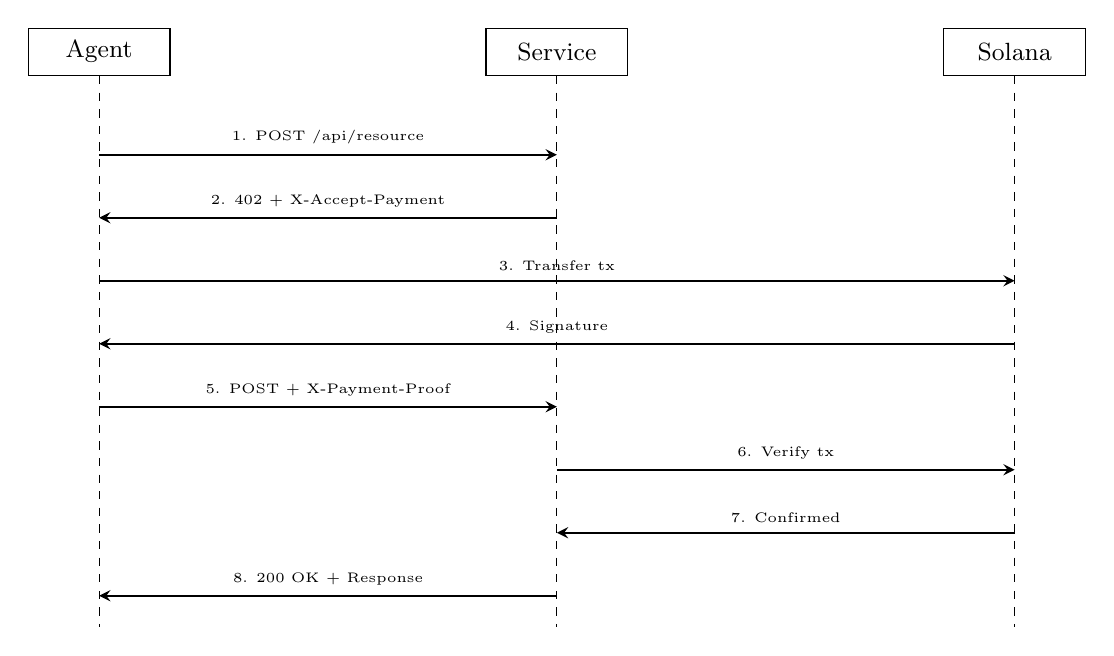
\begin{tikzpicture}[
    node distance=0.8cm,
    actor/.style={rectangle, draw, minimum width=1.8cm, minimum height=0.6cm, text centered, font=\small},
    msg/.style={->, >=stealth, thick},
    note/.style={font=\tiny, text width=3cm, align=center}
]
    % Actors
    \node[actor] (agent) {Agent};
    \node[actor, right=4cm of agent] (service) {Service};
    \node[actor, right=4cm of service] (solana) {Solana};
    
    % Lifelines
    \draw[dashed] (agent.south) -- ++(0,-7);
    \draw[dashed] (service.south) -- ++(0,-7);
    \draw[dashed] (solana.south) -- ++(0,-7);
    
    % Messages
    \draw[msg] ([yshift=-1cm]agent.south) -- ([yshift=-1cm]service.south) 
        node[midway, above, font=\tiny] {1. POST /api/resource};
    
    \draw[msg] ([yshift=-1.8cm]service.south) -- ([yshift=-1.8cm]agent.south) 
        node[midway, above, font=\tiny] {2. 402 + X-Accept-Payment};
    
    \draw[msg] ([yshift=-2.6cm]agent.south) -- ([yshift=-2.6cm]solana.south) 
        node[midway, above, font=\tiny] {3. Transfer tx};
    
    \draw[msg] ([yshift=-3.4cm]solana.south) -- ([yshift=-3.4cm]agent.south) 
        node[midway, above, font=\tiny] {4. Signature};
    
    \draw[msg] ([yshift=-4.2cm]agent.south) -- ([yshift=-4.2cm]service.south) 
        node[midway, above, font=\tiny] {5. POST + X-Payment-Proof};
    
    \draw[msg] ([yshift=-5cm]service.south) -- ([yshift=-5cm]solana.south) 
        node[midway, above, font=\tiny] {6. Verify tx};
    
    \draw[msg] ([yshift=-5.8cm]solana.south) -- ([yshift=-5.8cm]service.south) 
        node[midway, above, font=\tiny] {7. Confirmed};
    
    \draw[msg] ([yshift=-6.6cm]service.south) -- ([yshift=-6.6cm]agent.south) 
        node[midway, above, font=\tiny] {8. 200 OK + Response};
\end{tikzpicture}
\end{center}

\begin{center}
\small\textit{Figure 2: x402 Payment Flow. Agent receives 402, pays on-chain, then retries with proof.}
\end{center}

\subsection{Protocol Design}

\subsubsection{Payment Request}

When a service requires payment, it responds with HTTP 402 and an \texttt{X-Accept-Payment} header:

\begin{lstlisting}[language=HTTP,caption=HTTP 402 Payment Required Response]
HTTP/1.1 402 Payment Required
X-Accept-Payment: <base64-encoded-payment-request>
Content-Type: application/json

{
    "error": "payment_required",
    "message": "This endpoint requires payment"
}
\end{lstlisting}

The payment request (base64-decoded) contains:

\begin{lstlisting}[language=JSON,caption=Payment Request Structure]
{
    "version": "x0-v1",
    "recipient": "7xKXtg2CW87d97TXJSDpbD5jBkheTqA83TZRuJosgAsU",
    "amount": "1000000",
    "resource": "/api/v1/generate",
    "memo": "Text generation request",
    "network": "solana-mainnet",
    "escrow": {
        "use_escrow": false,
        "delivery_timeout": 3600,
        "auto_release_delay": 86400,
        "arbiter": null
    }
}
\end{lstlisting}

\subsubsection{Payment Proof}

After payment, the agent includes proof in subsequent requests:

\begin{lstlisting}[language=HTTP,caption=HTTP Request with Payment Proof]
POST /api/v1/generate HTTP/1.1
X-Payment-Proof: <base64-encoded-proof>
X-Payment-Version: x0-v1
Content-Type: application/json

{
    "prompt": "Generate a haiku about blockchain"
}
\end{lstlisting}

Payment proof contains:

\begin{lstlisting}[language=JSON,caption=Payment Proof Structure]
{
    "signature": "5VDx8F...",  // Transaction signature
    "slot": 123456789,
    "payer": "9xQeWv...",
    "timestamp": 1706400000,
    "network": "solana-mainnet"
}
\end{lstlisting}

\subsubsection{Verification}

The service verifies payment:

\begin{enumerate}
    \item Fetch transaction by signature
    \item Verify transaction succeeded
    \item Check recipient matches service wallet
    \item Check amount $\geq$ requested amount
    \item Verify timestamp within tolerance (±5 minutes)
    \item Check memo matches request (via SHA-256)
\end{enumerate}

\subsection{Security Properties}

\begin{theorem}[Payment Non-Repudiation]
A valid payment proof is unforgeable. An adversary cannot construct a proof without executing the on-chain transaction.
\end{theorem}

\begin{proof}
The proof contains transaction signature $\sigma = \texttt{Sign}(sk_A, tx)$. By existential unforgeability of Ed25519, an adversary cannot produce $\sigma'$ such that $\texttt{Verify}(pk_A, tx, \sigma') = 1$ without $sk_A$. On-chain verification ensures the transaction executed. \qed
\end{proof}

\section{Conditional Escrow (x0-escrow)}

\subsection{Design}

Escrow enables trustless payments for services with uncertain delivery.

\subsubsection{Escrow State Machine}

\begin{center}
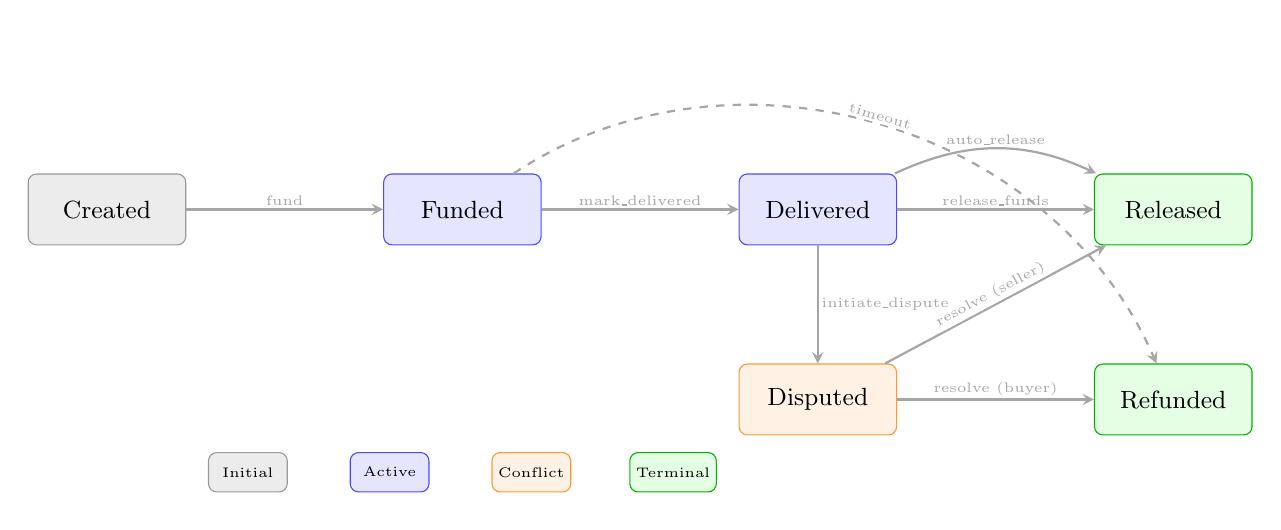
\begin{tikzpicture}[
    node distance=1.8cm and 2.5cm,
    % State styles with colors
    initial/.style={rectangle, rounded corners=3pt, draw=gray!80, fill=gray!15, 
        minimum width=2cm, minimum height=0.9cm, text centered, font=\small},
    active/.style={rectangle, rounded corners=3pt, draw=blue!70, fill=blue!10, 
        minimum width=2cm, minimum height=0.9cm, text centered, font=\small},
    conflict/.style={rectangle, rounded corners=3pt, draw=orange!80, fill=orange!10, 
        minimum width=2cm, minimum height=0.9cm, text centered, font=\small},
    terminal/.style={rectangle, rounded corners=3pt, draw=green!70!black, fill=green!10, 
        minimum width=2cm, minimum height=0.9cm, text centered, font=\small},
    % Arrow style
    arrow/.style={->, >=stealth, thick, color=gray!70},
    label/.style={font=\tiny, fill=white, inner sep=1pt}
]
    % States - arranged in logical flow
    \node[initial] (created) {Created};
    \node[active, right=of created] (funded) {Funded};
    \node[active, right=of funded] (delivered) {Delivered};
    \node[conflict, below=1.5cm of delivered] (disputed) {Disputed};
    \node[terminal, right=of delivered] (released) {Released};
    \node[terminal, below=1.5cm of released] (refunded) {Refunded};
    
    % Happy path (top row)
    \draw[arrow] (created) -- (funded) node[label, midway, above] {fund};
    \draw[arrow] (funded) -- (delivered) node[label, midway, above] {mark\_delivered};
    \draw[arrow] (delivered) -- (released) node[label, midway, above] {release\_funds};
    
    % Auto-release path
    \draw[arrow, bend left=25] (delivered) to node[label, above, sloped] {auto\_release} (released);
    
    % Dispute path
    \draw[arrow] (delivered) -- (disputed) node[label, midway, right] {initiate\_dispute};
    \draw[arrow] (disputed) -- (released) node[label, midway, above, sloped] {resolve (seller)};
    \draw[arrow] (disputed) -- (refunded) node[label, midway, above] {resolve (buyer)};
    
    % Timeout path
    \draw[arrow, dashed] (funded) to[bend left=50] node[label, above, sloped] {timeout} (refunded);
    
    % Legend
    \node[below=2.5cm of funded, font=\tiny] (legend) {
        \tikz{
            \node[initial, minimum width=1cm, minimum height=0.5cm, font=\tiny] at (0,0) {Initial};
            \node[active, minimum width=1cm, minimum height=0.5cm, font=\tiny] at (1.8,0) {Active};
            \node[conflict, minimum width=1cm, minimum height=0.5cm, font=\tiny] at (3.6,0) {Conflict};
            \node[terminal, minimum width=1cm, minimum height=0.5cm, font=\tiny] at (5.4,0) {Terminal};
        }
    };
\end{tikzpicture}
\end{center}

\begin{center}
\small\textit{Figure 3: Escrow State Machine. States are colored by type: gray (initial), blue (active), orange (conflict), green (terminal).}
\end{center}

\subsubsection{Escrow Account}

\begin{lstlisting}[language=Rust,caption=Escrow Account Structure]
#[account]
pub struct EscrowAccount {
    pub version: u8,                // Account version
    pub buyer: Pubkey,
    pub seller: Pubkey,
    pub arbiter: Option<Pubkey>,
    pub amount: u64,
    pub memo_hash: [u8; 32],
    pub state: EscrowState,
    pub timeout: i64,
    pub created_at: i64,
    pub delivery_proof: Option<[u8; 32]>,
    pub dispute_evidence: Option<[u8; 32]>,
    pub mint: Pubkey,
    pub token_decimals: u8,
    pub dispute_initiated_slot: u64,
    pub protocol_fee_paid: u64,     // Fee paid on creation
    pub bump: u8,
}
\end{lstlisting}

\subsection{Key Operations}

\subsubsection{Create and Fund}

\begin{algorithm}
\caption{Create and Fund Escrow}
\begin{algorithmic}[1]
\Procedure{CreateEscrow}{$B, S, A, x, m, \tau$}
    \State \textbf{require} $B \neq S$
    \State \textbf{require} $3600 \leq \tau \leq 2592000$ \Comment{1h to 30d}
    \State $e \gets \texttt{EscrowPDA}(B, S, H(m))$
    \State $e.\texttt{timeout} \gets t_{\text{now}} + \tau$
    \State $e.\texttt{state} \gets \texttt{Created}$
    \State \Return $e$
\EndProcedure
\Procedure{FundEscrow}{$e, x$}
    \State \textbf{require} $e.\texttt{state} = \texttt{Created}$
    \State \textbf{require} $t_{\text{now}} < e.\texttt{timeout}$
    \State $\texttt{transfer}(B, e, x)$
    \State $e.\texttt{state} \gets \texttt{Funded}$
\EndProcedure
\end{algorithmic}
\end{algorithm}

\subsubsection{Delivery and Release}

\begin{algorithm}
\caption{Mark Delivered and Release Funds}
\begin{algorithmic}[1]
\Procedure{MarkDelivered}{$e, p$}
    \State \textbf{require} $\texttt{signer} = e.\texttt{seller}$
    \State \textbf{require} $e.\texttt{state} = \texttt{Funded}$
    \State $e.\texttt{delivery\_proof} \gets H(p)$
    \State $e.\texttt{state} \gets \texttt{Delivered}$
\EndProcedure
\Procedure{ReleaseFunds}{$e$}
    \State \textbf{require} $\texttt{signer} = e.\texttt{buyer}$
    \State \textbf{require} $e.\texttt{state} = \texttt{Delivered}$
    \State $e.\texttt{state} \gets \texttt{Released}$ \Comment{BEFORE transfer!}
    \State $\texttt{transfer}(e, e.\texttt{seller}, e.\texttt{amount})$
    \State $\texttt{UpdateReputation}(e.\texttt{seller}, \texttt{Success})$ \Comment{Optional CPI}
\EndProcedure
\end{algorithmic}
\end{algorithm}

\subsubsection{Auto-Release}

After delivery, if buyer doesn't dispute within timeout, seller can claim:

\begin{algorithm}
\caption{Auto-Release After Timeout}
\begin{algorithmic}[1]
\Procedure{ClaimAutoRelease}{$e$}
    \State \textbf{require} $\texttt{signer} = e.\texttt{seller}$
    \State \textbf{require} $e.\texttt{state} = \texttt{Delivered}$
    \State \textbf{require} $t_{\text{now}} > e.\texttt{timeout}$
    \State $e.\texttt{state} \gets \texttt{Released}$
    \State $\texttt{transfer}(e, e.\texttt{seller}, e.\texttt{amount})$
    \State $\texttt{UpdateReputation}(e.\texttt{seller}, \texttt{Success})$
\EndProcedure
\end{algorithmic}
\end{algorithm}

\subsubsection{Dispute Resolution}

\begin{algorithm}
\caption{Initiate and Resolve Dispute}
\begin{algorithmic}[1]
\Procedure{InitiateDispute}{$e, d$}
    \State \textbf{require} $\texttt{signer} \in \{e.\texttt{buyer}, e.\texttt{seller}\}$
    \State \textbf{require} $e.\texttt{state} = \texttt{Delivered}$
    \State $e.\texttt{dispute\_evidence} \gets H(d)$
    \State $e.\texttt{dispute\_initiated\_slot} \gets \texttt{current\_slot}$
    \State $e.\texttt{state} \gets \texttt{Disputed}$
    \State $\texttt{UpdateReputation}(e.\texttt{seller}, \texttt{Dispute})$
\EndProcedure
\Procedure{ResolveDispute}{$e, \texttt{release\_to\_seller}$}
    \State \textbf{require} $\texttt{signer} = e.\texttt{arbiter}$
    \State \textbf{require} $e.\texttt{state} = \texttt{Disputed}$
    \State \textbf{require} $\texttt{current\_slot} \geq e.\texttt{dispute\_initiated\_slot} + \Delta$
    \State \Comment{$\Delta = 216000$ slots $\approx$ 24 hours}
    \If{$\texttt{release\_to\_seller}$}
        \State $e.\texttt{state} \gets \texttt{Released}$
        \State $\texttt{transfer}(e, e.\texttt{seller}, e.\texttt{amount})$
        \State $\texttt{UpdateReputation}(e.\texttt{seller}, \texttt{ResolutionFavor})$
    \Else
        \State $e.\texttt{state} \gets \texttt{Refunded}$
        \State $\texttt{transfer}(e, e.\texttt{buyer}, e.\texttt{amount})$
    \EndIf
\EndProcedure
\end{algorithmic}
\end{algorithm}

\subsection{Security Analysis}

\begin{theorem}[Escrow Safety]
An escrow satisfies:
\begin{enumerate}
    \item \textbf{Atomicity}: Funds are either fully released or refunded, never partially
    \item \textbf{Liveness}: Funds are never permanently locked
    \item \textbf{Fairness}: Either party can initiate dispute; arbiter is neutral
\end{enumerate}
\end{theorem}

\begin{proof}
\textbf{Atomicity}: State transitions are atomic. The \texttt{Released} and \texttt{Refunded} states are terminal.

\textbf{Liveness}: Three exit paths exist:
\begin{itemize}
    \item Buyer releases after delivery
    \item Seller claims auto-release after timeout
    \item Arbiter resolves dispute
\end{itemize}
At least one path is always available after delivery or timeout.

\textbf{Fairness}: Either party can initiate dispute. Arbiter resolution requires evidence from both parties and a 24-hour delay. \qed
\end{proof}

\section{Reputation Oracle (x0-reputation)}

\subsection{Design Goals}

\begin{enumerate}
    \item \textbf{Transparency}: All reputation data on-chain
    \item \textbf{Temporal Decay}: Old successes shouldn't dominate forever
    \item \textbf{Sybil Resistance}: New agents don't get perfect scores
    \item \textbf{Nuanced Scoring}: Distinguish success, failure, disputes, resolutions
\end{enumerate}

\subsection{Reputation Account}

\begin{lstlisting}[language=Rust,caption=Reputation Account Structure]
#[account]
pub struct AgentReputation {
    pub version: u8,                   // Account version (v2)
    pub agent_id: Pubkey,
    pub total_transactions: u64,
    pub successful_transactions: u64,
    pub disputed_transactions: u64,
    pub resolved_in_favor: u64,
    pub failed_transactions: u64,      // Policy rejections
    pub average_response_time_ms: u32,
    pub cumulative_response_time_ms: u64,
    pub last_updated: i64,
    pub last_decay_applied: i64,
    pub bump: u8,
}
\end{lstlisting}

\subsection{Reputation Score Calculation}

\begin{definition}[Reputation Score]
The reputation score $S \in [0, 1]$ is computed as:
\begin{align}
S &= 0.60 \cdot S_{\text{success}} + 0.15 \cdot S_{\text{resolution}} \nonumber \\
&\quad + 0.10 \cdot (1 - R_{\text{dispute}}) + 0.15 \cdot (1 - R_{\text{failure}})
\end{align}
where:
\begin{align}
S_{\text{success}} &= \frac{n_{\text{success}}}{n_{\text{total}}} \\
S_{\text{resolution}} &= \begin{cases}
\frac{n_{\text{resolved}}}{n_{\text{disputed}}} & n_{\text{disputed}} > 0 \\
0.5 & n_{\text{disputed}} = 0 \land n_{\text{total}} < 10 \\
1.0 & n_{\text{disputed}} = 0 \land n_{\text{total}} \geq 10
\end{cases} \\
R_{\text{dispute}} &= \frac{n_{\text{disputed}}}{n_{\text{total}}} \\
R_{\text{failure}} &= \frac{n_{\text{failed}}}{n_{\text{total}}}
\end{align}
\end{definition}

\begin{remark}
The neutral resolution score (0.5) for new agents prevents Sybil attacks where attackers create new identities to get perfect scores.
\end{remark}

\begin{example}[Reputation Score Calculation]
Consider an agent with the following transaction history:
\begin{itemize}
    \item Total transactions: $n_{\text{total}} = 100$
    \item Successful: $n_{\text{success}} = 90$
    \item Disputed: $n_{\text{disputed}} = 5$
    \item Resolved in favor: $n_{\text{resolved}} = 3$
    \item Failed (policy rejections): $n_{\text{failed}} = 2$
\end{itemize}

Computing component scores:
\begin{align*}
S_{\text{success}} &= \frac{90}{100} = 0.90 \\
S_{\text{resolution}} &= \frac{3}{5} = 0.60 \quad (\text{since } n_{\text{disputed}} > 0) \\
R_{\text{dispute}} &= \frac{5}{100} = 0.05 \\
R_{\text{failure}} &= \frac{2}{100} = 0.02
\end{align*}

Final reputation score:
\begin{align*}
S &= 0.60(0.90) + 0.15(0.60) + 0.10(1 - 0.05) + 0.15(1 - 0.02) \\
&= 0.540 + 0.090 + 0.095 + 0.147 \\
&= \mathbf{0.872}
\end{align*}

This agent has a strong reputation (87.2\%), with room for improvement in dispute resolution.
\end{example}

\subsection{Temporal Decay}

\begin{definition}[Exponential Decay]
Monthly decay applies to successful transactions:
\begin{equation}
n_{\text{success}}^{(t+1)} = n_{\text{success}}^{(t)} \cdot (1 - \alpha)
\end{equation}
where $\alpha = 0.01$ (1\% monthly decay) and $t$ is measured in months.
\end{definition}

For $m$ months:
\begin{equation}
n_{\text{success}}^{(t+m)} = n_{\text{success}}^{(t)} \cdot (0.99)^m
\end{equation}

\begin{proposition}[Half-Life]
The half-life of reputation is:
\begin{equation}
t_{1/2} = \frac{\ln 2}{\ln(1/0.99)} \approx 69 \text{ months}
\end{equation}
\end{proposition}

\begin{algorithm}
\caption{Apply Reputation Decay}
\begin{algorithmic}[1]
\Procedure{ApplyDecay}{$r$}
    \State $m \gets \lfloor (t_{\text{now}} - r.\texttt{last\_decay\_applied}) / 2592000 \rfloor$
    \If{$m > 0$}
        \State $d_{\text{mult}} \gets 99^{\min(m, 12)}$ \Comment{Cap at 12 months}
        \State $d_{\text{div}} \gets 100^{\min(m, 12)}$
        \State $r.\texttt{successful\_transactions} \gets r.\texttt{successful\_transactions} \cdot d_{\text{mult}} / d_{\text{div}}$
        \State $r.\texttt{last\_decay\_applied} \gets t_{\text{now}}$
    \EndIf
\EndProcedure
\end{algorithmic}
\end{algorithm}

\subsection{Authorization Model}

\begin{definition}[Authorized Callers]
Reputation updates can only be called by:
\begin{itemize}
    \item \textbf{Escrow program}: Records success/dispute/resolution
    \item \textbf{Guard program}: Records policy failures
    \item \textbf{Policy owner}: Self-reported off-chain transactions
\end{itemize}
\end{definition}

\begin{theorem}[Reputation Integrity]
An adversary cannot artificially inflate reputation without:
\begin{enumerate}
    \item Completing escrow transactions (requires payment)
    \item Winning disputes (requires arbiter approval)
    \item Controlling policy owner key (equivalent to ownership)
\end{enumerate}
\end{theorem}

\section{Agent Discovery (x0-registry)}

\subsection{Registry Entry}

\begin{lstlisting}[language=Rust,caption=Registry Entry Structure]
#[account]
pub struct AgentRegistry {
    pub version: u8,                   // Account version
    pub agent_id: Pubkey,
    pub owner: Pubkey,
    pub endpoint: String,              // Max 256 chars
    pub capabilities: Vec<Capability>, // Max 10 capabilities
    pub metadata_uri: Option<String>,  // Extended metadata
    pub price_oracle: Option<Pubkey>,
    pub reputation_pda: Option<Pubkey>,
    pub min_transaction_amount: u64,
    pub max_transaction_amount: Option<u64>,
    pub supported_tokens: Vec<Pubkey>, // Max 5 tokens
    pub last_updated: i64,
    pub created_at: i64,
    pub total_transactions: u64,
    pub is_active: bool,
    pub is_verified: bool,             // Protocol verification
    pub bump: u8,
}

pub struct Capability {
    pub capability_type: String,       // Max 64 chars
    pub version: String,               // Max 32 chars
    pub price_lamports: u64,
    pub metadata: String,              // Max 256 chars
}
\end{lstlisting}

\subsection{Discovery Algorithm}

\begin{algorithm}
\caption{Find Agents by Capability}
\begin{algorithmic}[1]
\Procedure{FindAgents}{$\texttt{cap\_type}$}
    \State $A \gets \{\}$ \Comment{Set of matching agents}
    \For{$e \in \texttt{GetProgramAccounts}(\texttt{registry\_program})$}
        \If{$\texttt{cap\_type} \in e.\texttt{capabilities} \land e.\texttt{is\_active}$}
            \State $s \gets \texttt{FetchReputation}(e.\texttt{reputation\_pda})$
            \State $A \gets A \cup \{(e, s)\}$
        \EndIf
    \EndFor
    \State \Return $\texttt{SortByScore}(A)$
\EndProcedure
\end{algorithmic}
\end{algorithm}

\subsection{Capability Metadata}

Capabilities use JSON metadata:

\begin{lstlisting}[language=JSON,caption=Capability Metadata Example]
{
    "type": "text-generation",
    "models": ["gpt-4", "claude-3"],
    "pricing": {
        "per_token": 0.00001,
        "minimum": 0.01
    },
    "rate_limit": {
        "requests_per_minute": 60,
        "burst": 10
    },
    "api_version": "v1"
}
\end{lstlisting}

\section{USDC Wrapper (x0-wrapper)}

\subsection{Problem Statement}

Direct USDC usage has limitations:
\begin{enumerate}
    \item No transfer hook support on standard USDC
    \item Different token programs (SPL vs Token-2022)
    \item Protocol fees require wrapper
\end{enumerate}

\subsection{Design}

x0-USD is a 1:1 USDC-backed Token-2022 token with:
\begin{itemize}
    \item Transfer hook pointing to x0-guard
    \item 0.8\% transfer fee (configurable via \texttt{PROTOCOL\_FEE\_BASIS\_POINTS} constant, default 80 bps)
    \item Configurable redemption fee (default 0.8\%, set via \texttt{WRAPPER\_REDEMPTION\_FEE\_BPS})
\end{itemize}

\subsubsection{Reserve Invariant}

\begin{definition}[Reserve Invariant]
At all times, the following must hold:
\begin{equation}
R_{\text{USDC}} \geq S_{\text{x0-USD}}
\end{equation}
where $R_{\text{USDC}}$ is USDC reserve and $S_{\text{x0-USD}}$ is outstanding x0-USD supply.
\end{definition}

\begin{theorem}[Invariant Preservation]
The reserve invariant is preserved under all operations.
\end{theorem}

\begin{proof}
We prove by cases:

\textbf{Deposit}: User deposits $x$ USDC, receives $x$ x0-USD.
\begin{equation}
R' = R + x, \quad S' = S + x \implies R' - S' = R - S \geq 0
\end{equation}

\textbf{Redemption}: User burns $x$ x0-USD, receives $x - f$ USDC (fee $f$).
\begin{equation}
R' = R - (x - f), \quad S' = S - x
\end{equation}
\begin{equation}
R' - S' = R - x + f - S + x = R - S + f \geq R - S \geq 0
\end{equation}

The fee increases the reserve ratio. \qed
\end{proof}

\subsection{Governance}

\subsubsection{Timelock}

All admin operations require 48-hour timelock:

\begin{algorithm}
\caption{Timelock Pattern}
\begin{algorithmic}[1]
\Procedure{ScheduleAction}{$a, v, t$}
    \State $\texttt{action\_pda} \gets \texttt{CreateActionPDA}(a, \texttt{nonce})$
    \State $\texttt{action\_pda.type} \gets a$
    \State $\texttt{action\_pda.value} \gets v$
    \State $\texttt{action\_pda.scheduled\_time} \gets t + 172800$ \Comment{48h}
\EndProcedure
\Procedure{ExecuteAction}{$\texttt{action\_pda}$}
    \State \textbf{require} $t_{\text{now}} \geq \texttt{action\_pda.scheduled\_time}$
    \State \textbf{require} $\neg \texttt{action\_pda.executed}$
    \State \textbf{require} $\neg \texttt{action\_pda.cancelled}$
    \State $\texttt{ApplyAction}(\texttt{action\_pda.type}, \texttt{action\_pda.value})$
    \State $\texttt{action\_pda.executed} \gets \texttt{true}$
\EndProcedure
\end{algorithmic}
\end{algorithm}

\subsubsection{Emergency Pause}

Emergency pause is the \textbf{only} operation bypassing timelock:
\begin{itemize}
    \item Can only \textbf{pause}, never unpause
    \item Unpausing requires standard timelock
    \item Prevents rapid pause/unpause attacks
\end{itemize}

\subsection{Reserve Ratio Monitoring}

\begin{definition}[Reserve Ratio]
\begin{equation}
\rho = \frac{R_{\text{USDC}}}{S_{\text{x0-USD}}}
\end{equation}
\end{definition}

Alert levels:
\begin{itemize}
    \item $\rho < 1.01$: Warning alert
    \item $\rho < 1.00$: Critical alert (undercollateralized)
\end{itemize}

\section{Human-in-the-Loop (Blinks)}

\subsection{Problem Statement}

Full automation is dangerous for:
\begin{enumerate}
    \item Transfers exceeding daily limit
    \item Recipients not on whitelist
    \item Unusually large transactions
\end{enumerate}

\subsection{Blink Design}

A \textbf{Blink} is a Solana Action requesting human approval.

\subsubsection{Generation}

When guard rejects a transfer due to limits, it can:
\begin{enumerate}
    \item Generate Blink ID: $b = H(\texttt{policy} \parallel R \parallel x \parallel t)[0..16]$
    \item Emit \texttt{BlinkGenerated} event with:
    \begin{itemize}
        \item Blink ID
        \item Requested amount
        \item Recipient
        \item Expiration (15 minutes)
    \end{itemize}
    \item Charge fee (0.001 SOL) to prevent spam
\end{enumerate}

\subsubsection{Rate Limiting}

\begin{definition}[Blink Rate Limit]
Maximum 3 Blinks per hour per policy.
\end{definition}

\begin{algorithm}
\caption{Blink Rate Limit Check}
\begin{algorithmic}[1]
\Procedure{CheckBlinkRateLimit}{$p, t$}
    \State $h_{\text{current}} \gets \lfloor t / 3600 \rfloor$
    \State $h_{\text{window}} \gets \lfloor p.\texttt{blink\_hour\_start} / 3600 \rfloor$
    \If{$h_{\text{current}} \neq h_{\text{window}}$}
        \State $p.\texttt{blink\_hour\_start} \gets t$
        \State $p.\texttt{blinks\_this\_hour} \gets 0$
    \EndIf
    \If{$p.\texttt{blinks\_this\_hour} \geq 3$}
        \State \Return \texttt{false}
    \EndIf
    \State $p.\texttt{blinks\_this\_hour} \gets p.\texttt{blinks\_this\_hour} + 1$
    \State \Return \texttt{true}
\EndProcedure
\end{algorithmic}
\end{algorithm}

\subsubsection{Approval}

Owner approves via:
\begin{enumerate}
    \item Viewing Blink details (QR code, web interface, wallet)
    \item Signing approval transaction
    \item Temporarily raising limit or whitelisting recipient
\end{enumerate}

\section{Economic Model}

\subsection{Fee Structure}

\begin{table}[h]
\centering
\begin{tabular}{|l|l|l|}
\hline
\textbf{Operation} & \textbf{Fee} & \textbf{Recipient} \\
\hline
Transfer (x0-USD) & 0.8\% & Protocol treasury \\
Registry listing & 0.1 SOL & Protocol treasury \\
Blink generation & 0.001 SOL & Protocol treasury \\
Wrapper redemption & 0.8\% (configurable) & Wrapper reserve \\
\hline
\end{tabular}
\caption{Protocol Fee Schedule}
\end{table}

\subsection{Fee Collection}

Transfer fees are collected via Token-2022's TransferFee extension:

\begin{algorithm}
\caption{Fee Harvesting}
\begin{algorithmic}[1]
\Procedure{HarvestFees}{$\texttt{mint}, \texttt{accounts}$}
    \For{$a \in \texttt{accounts}$}
        \State $f \gets \texttt{GetWithheldAmount}(a)$
        \State $\texttt{TransferWithheldToMint}(a, f)$
    \EndFor
    \State $F \gets \sum_a f$
    \State $\texttt{WithdrawWithheldFromMint}(\texttt{mint}, \texttt{treasury}, F)$
\EndProcedure
\end{algorithmic}
\end{algorithm}

\subsection{Token Economics}

\subsubsection{x0-USD Supply Dynamics}

\begin{align}
\frac{dS}{dt} &= D(t) - R(t) \\
\frac{dR_{\text{USDC}}}{dt} &= D(t) - R(t) + f \cdot R(t)
\end{align}

where:
\begin{itemize}
    \item $S(t)$ = x0-USD supply
    \item $R_{\text{USDC}}(t)$ = USDC reserve
    \item $D(t)$ = Deposit rate
    \item $R(t)$ = Redemption rate (before fees)
    \item $f$ = Redemption fee rate
\end{itemize}

Reserve ratio evolution:
\begin{equation}
\rho(t) = \frac{R_{\text{USDC}}(t)}{S(t)} = 1 + \int_0^t \frac{f \cdot R(\tau)}{S(\tau)} d\tau
\end{equation}

The reserve ratio increases over time due to fees.

\section{Security Analysis}

\subsection{Threat Model}

We consider the following adversaries:

\begin{enumerate}
    \item \textbf{Compromised Agent}: Attacker obtains $sk_A$
    \item \textbf{Malicious Service}: Service provider attempts fraud
    \item \textbf{Malicious Agent}: Agent attempts reputation manipulation
    \item \textbf{Wrapper Attack}: Attacker attempts reserve drain
\end{enumerate}

\subsection{Attack Scenarios and Mitigations}

\subsubsection{Compromised Agent Key}

\textbf{Attack}: Adversary steals $sk_A$, attempts unlimited spending.

\textbf{Mitigation}: 
\begin{itemize}
    \item Rolling window limits spending to $L$ per 24 hours
    \item Owner can revoke via \texttt{revoke\_agent\_authority}
    \item Maximum loss bounded by $L + x_{\text{max}}$ where $x_{\text{max}}$ is max transaction size
\end{itemize}

\subsubsection{Sybil Attack on Reputation}

\textbf{Attack}: Adversary creates multiple identities to appear trustworthy.

\textbf{Mitigation}:
\begin{itemize}
    \item Registry listing costs 0.1 SOL
    \item New agents get neutral (0.5) resolution score, not perfect
    \item Temporal decay prevents dormant identities
\end{itemize}

Cost for 100 Sybil identities: $100 \times 0.1 = 10$ SOL $\approx \$1000$ (at \$100/SOL).

\subsubsection{Escrow Griefing}

\textbf{Attack}: Malicious buyer creates many escrows, ties up seller funds.

\textbf{Mitigation}:
\begin{itemize}
    \item Escrow creation is permissionless but buyer must fund
    \item Sellers can set minimum transaction amounts
    \item Reputation tracking penalizes frivolous disputes
\end{itemize}

\subsubsection{Wrapper Reserve Drain}

\textbf{Attack}: Exploit bug to withdraw USDC without burning x0-USD.

\textbf{Mitigation}:
\begin{itemize}
    \item Reserve invariant checked before every redemption
    \item State updated before transfer (reentrancy protection)
    \item Admin operations timelocked (48h notice)
    \item Emergency pause available
\end{itemize}

\subsubsection{Transfer Hook Configuration Attack}

\textbf{Attack}: Unauthorized party front-runs transfer hook initialization for a mint, potentially misconfiguring the extra account metas or consuming the PDA address.

\textbf{Mitigation}:
\begin{itemize}
    \item Only the Token-2022 mint authority can initialize extra account metas
    \item Re-initialization is blocked after first valid configuration
    \item Extra account metas configuration is deterministic (not caller-supplied)
    \item Mint authority verification uses \texttt{StateWithExtensions} for robust parsing
\end{itemize}

\textbf{Impact}: Even though the extra metas configuration is hardcoded in the program, preventing unauthorized initialization eliminates a griefing vector where an attacker could pay the rent and claim the PDA before the legitimate mint authority initializes it.

\subsection{Formal Verification}

\subsubsection{Spend Limit Invariant}

\begin{theorem}[Daily Spend Limit]
For all execution traces, if policy has daily limit $L$:
\begin{equation}
\forall t: \sum_{i: t_i > t - 86400} x_i \leq L
\end{equation}
\end{theorem}

\begin{proof}
Proven in Section 3.4. \qed
\end{proof}

\subsubsection{Reserve Invariant}

\begin{theorem}[Wrapper Reserve Invariant]
For all execution traces:
\begin{equation}
\forall t: R_{\text{USDC}}(t) \geq S_{\text{x0-USD}}(t)
\end{equation}
\end{theorem}

\begin{proof}
Proven in Section 7.2. \qed
\end{proof}

\section{Performance Analysis}

\subsection{Computational Complexity}

\begin{table}[h]
\centering
\begin{tabular}{|l|l|l|}
\hline
\textbf{Operation} & \textbf{Time} & \textbf{Space} \\
\hline
Transfer validation & $O(n)$ & $O(n)$ \\
Merkle verification & $O(\log m)$ & $O(\log m)$ \\
Bloom verification & $O(k)$ & $O(1)$ \\
Reputation update & $O(1)$ & $O(1)$ \\
Registry search & $O(N)$ & $O(1)$ \\
\hline
\end{tabular}
\caption{Computational Complexity ($n$ = window size, $m$ = whitelist size, $k$ = hash count, $N$ = registered agents)}
\end{table}

\subsection{On-Chain Costs}

\begin{table}[h]
\centering
\begin{tabular}{|l|l|l|}
\hline
\textbf{Account} & \textbf{Size (bytes)} & \textbf{Rent (SOL)} \\
\hline
AgentPolicy & 4,952 & 0.035 \\
EscrowAccount & 307 & 0.0030 \\
AgentRegistry & 2,064 & 0.015 \\
AgentReputation & 114 & 0.0016 \\
WrapperConfig & 243 & 0.0025 \\
\hline
\end{tabular}
\caption{Account Sizes and Rent Costs (at 0.00000348 SOL/byte-epoch)}
\end{table}

\subsection{Transaction Benchmarks}

Measured on Solana devnet (February 2026):

\begin{table}[h]
\centering
\begin{tabular}{|l|l|l|}
\hline
\textbf{Operation} & \textbf{Compute Units} & \textbf{Latency} \\
\hline
Initialize policy & 45,000 & 450ms \\
Validate transfer (Merkle) & 32,000 & 320ms \\
Validate transfer (Bloom) & 18,000 & 180ms \\
Create escrow & 28,000 & 280ms \\
Registry listing & 35,000 & 350ms \\
Reputation update & 15,000 & 150ms \\
\hline
\end{tabular}
\caption{Transaction Performance (1 CU $\approx$ 10 µs)}
\end{table}

\section{Related Work}

\subsection{Payment Channels}

Bitcoin's Lightning Network \cite{lightning} and Ethereum's Raiden \cite{raiden} enable off-chain micropayments. Limitations:
\begin{itemize}
    \item Require channel opening/closing (on-chain)
    \item Liquidity fragmentation
    \item Limited programmability
\end{itemize}

x0 uses on-chain transactions but adds programmable policy enforcement unavailable in payment channels.

\subsection{Escrow Protocols}

Traditional escrow (e.g., Escrow.com) requires trusted third parties. Smart contract escrow (OpenBazaar, LocalBitcoins) removes intermediaries but lacks:
\begin{itemize}
    \item Reputation integration
    \item Automated dispute resolution
    \item Cross-protocol standards
\end{itemize}

\subsection{Reputation Systems}

OpenBazaar and Augur implement on-chain reputation but lack:
\begin{itemize}
    \item Temporal decay
    \item Sybil resistance for new participants
    \item Integration with payment protocols
\end{itemize}

x0's reputation oracle addresses these limitations.

\section{Future Work}

\subsection{Zero-Knowledge Proofs}

Future versions may use ZK-SNARKs for:
\begin{itemize}
    \item Private spend limit verification
    \item Proof of reputation without revealing details
    \item Confidential escrow amounts
\end{itemize}

\subsection{Cross-Chain Support}

Extend to other chains via:
\begin{itemize}
    \item Wormhole integration for cross-chain messages
    \item Unified reputation across chains
    \item Cross-chain escrow settlement
\end{itemize}

\subsection{Machine Learning Integration}

\begin{itemize}
    \item Anomaly detection for suspicious agent behavior
    \item Dynamic reputation weighting
    \item Predictive escrow dispute resolution
\end{itemize}

\subsection{Governance}

\begin{itemize}
    \item DAO for protocol parameter updates
    \item Community-driven arbiter selection
    \item Fee redistribution to token holders
\end{itemize}

\section{Conclusion}

We have presented x0, a comprehensive payment infrastructure for autonomous agents. The protocol's key innovations include:

\begin{enumerate}
    \item \textbf{Transfer Hook Policy Enforcement}: Programmable spending limits enforced cryptographically on every transaction
    \item \textbf{HTTP 402 Protocol}: Standardized payment negotiation for agent-to-agent commerce
    \item \textbf{Conditional Escrow}: Trustless high-value transactions with dispute resolution
    \item \textbf{Temporal Reputation}: On-chain trust scores with decay to prevent stale reputations
    \item \textbf{USDC Wrapper}: Stable payments with cryptographic reserve invariants
    \item \textbf{Human-in-the-Loop}: Fallback mechanism for exceptional cases
\end{enumerate}

The protocol has been deployed on Solana devnet and is undergoing security audits. We invite the community to review the codebase at \texttt{github.com/x0-protocol} and provide feedback.

The future of AI agent commerce requires infrastructure that is:
\begin{itemize}
    \item \textbf{Fast}: Sub-second transaction finality
    \item \textbf{Cheap}: Sub-cent transaction costs
    \item \textbf{Programmable}: Enforcing complex spending rules
    \item \textbf{Trustless}: No centralized intermediaries
    \item \textbf{Safe}: Bounded downside risk
\end{itemize}

x0 achieves these properties through careful cryptographic design and integration with Solana's high-performance blockchain.

\section*{Acknowledgments}

We thank the Solana Foundation for technical support, the Anchor framework team for excellent developer tooling, and the broader Solana community for feedback during development. Special thanks to the auditors at OtterSec and Trail of Bits for security reviews.

\begin{thebibliography}{99}

\bibitem{bitcoin}
Nakamoto, S. (2008). Bitcoin: A Peer-to-Peer Electronic Cash System.

\bibitem{ethereum}
Buterin, V. (2014). Ethereum: A Next-Generation Smart Contract and Decentralized Application Platform.

\bibitem{solana}
Yakovenko, A. (2018). Solana: A new architecture for a high performance blockchain.

\bibitem{lightning}
Poon, J., \& Dryja, T. (2016). The Bitcoin Lightning Network: Scalable Off-Chain Instant Payments.

\bibitem{raiden}
Raiden Network Team. (2017). Raiden Network: Fast, cheap, scalable token transfers for Ethereum.

\bibitem{token22}
Solana Labs. (2023). Token-2022 Extension Documentation. \url{https://spl.solana.com/token-2022}

\bibitem{elgamal}
ElGamal, T. (1985). A public key cryptosystem and a signature scheme based on discrete logarithms. IEEE Transactions on Information Theory, 31(4), 469-472.

\bibitem{merkle}
Merkle, R. C. (1988). A Digital Signature Based on a Conventional Encryption Function. CRYPTO '87.

\bibitem{bloom}
Bloom, B. H. (1970). Space/time trade-offs in hash coding with allowable errors. Communications of the ACM, 13(7), 422-426.

\bibitem{ed25519}
Bernstein, D. J., et al. (2012). High-speed high-security signatures. Journal of Cryptographic Engineering, 2(2), 77-89.

\end{thebibliography}

\appendix

\section{Error Codes Reference}

\begin{table}[h]
\centering
\small
\begin{tabular}{|l|l|l|}
\hline
\textbf{Code} & \textbf{Name} & \textbf{Description} \\
\hline
\multicolumn{3}{|c|}{\textit{x0-common errors (0x1770+)}} \\
\hline
0x1770 & Unauthorized & Unauthorized access \\
0x1771 & InvalidAmount & Invalid amount specified \\
0x1772 & InvalidTimestamp & Invalid timestamp \\
0x1773 & AccountNotInitialized & Account not initialized \\
0x1774 & InvalidProgramId & Invalid program ID \\
0x1775 & MathOverflow & Math overflow error \\
0x1776 & InvalidMint & Invalid token mint \\
0x1777 & InsufficientFunds & Insufficient funds \\
0x1778 & InvalidState & Invalid state transition \\
0x1779 & Expired & Operation has expired \\
0x177A & NotExpired & Not yet expired \\
0x177B & AlreadyInitialized & Already initialized \\
0x177C & InvalidOwner & Invalid owner \\
0x177D & InvalidSigner & Invalid signer \\
0x177E & InvalidAccount & Invalid account \\
0x177F & InvalidInstruction & Invalid instruction \\
0x1780 & RateLimitExceeded & Rate limit exceeded \\
0x1781 & InvalidProof & Invalid cryptographic proof \\
0x1782 & InvalidHash & Invalid hash value \\
0x1783 & InvalidSignature & Invalid signature \\
0x1784 & InvalidPublicKey & Invalid public key \\
0x1785 & InvalidSeed & Invalid PDA seed \\
0x1786 & InvalidBump & Invalid PDA bump \\
0x1787 & InvalidData & Invalid account data \\
0x1788 & InvalidLength & Invalid data length \\
0x1789 & InvalidVersion & Invalid account version \\
\hline
\multicolumn{3}{|c|}{\textit{Guard-specific errors}} \\
\hline
0x178A & PolicyNotActive & Policy is deactivated \\
0x178B & DailyLimitExceeded & Transfer exceeds 24h limit \\
0x178C & SingleTxLimitExceeded & Exceeds per-tx limit \\
0x178D & DestinationNotWhitelisted & Recipient not in whitelist \\
0x178E & WindowOverflow & Rolling window overflow \\
0x178F & ExtraMetasAlreadyInit & Extra metas re-init blocked \\
0x1790 & UnauthorizedMetasInit & Mint authority required \\
\hline
\multicolumn{3}{|c|}{\textit{Escrow-specific errors}} \\
\hline
0x1791 & InvalidEscrowState & Invalid state transition \\
0x1792 & DisputeDelayNotMet & 24h dispute delay not met \\
0x1793 & ArbiterRequired & Arbiter required for dispute \\
\hline
\multicolumn{3}{|c|}{\textit{Wrapper-specific errors}} \\
\hline
0x1794 & WrapperPaused & Wrapper operations paused \\
0x1795 & InsufficientReserve & Reserve undercollateralized \\
0x1796 & TimelockNotExpired & Timelock period not expired \\
0x1797 & ActionAlreadyExecuted & Timelock action already executed \\
0x1798 & ActionCancelled & Timelock action was cancelled \\
\hline
\end{tabular}
\caption{Protocol Error Codes (Anchor offset: 6000 + index)}
\end{table}

\section{Program Addresses}

\begin{table}[h]
\centering
\begin{tabular}{|l|l|}
\hline
\textbf{Program} & \textbf{Devnet Address} \\
\hline
x0-guard & \texttt{2uYGW3fQUGfhrwVbkupdasXBpRPfGYBGTLUdaPTXU9vP} \\
x0-token & \texttt{EHHTCSyGkmnsBhGsvCmLzKgcSxtsN31ScrfiwcCbjHci} \\
x0-escrow & \texttt{AhaDyVm8LBxpUwFdArA37LnHvNx6cNWe3KAiy8zGqhHF} \\
x0-registry & \texttt{Bebty49EPhFoANKDw7TqLQ2bX61ackNav5iNkj36eVJo} \\
x0-reputation & \texttt{FfzkTWRGAJQPDePbujZdEhKHqC1UpqvDrpv4TEiWpx6y} \\
x0-wrapper & \texttt{EomiXBbg94Smu4ipDoJtuguazcd1KjLFDFJt2fCabvJ8} \\
\hline
\end{tabular}
\caption{Deployed Program Addresses}
\end{table}

\section{Mathematical Notation}

\begin{table}[h]
\centering
\begin{tabular}{|l|l|}
\hline
\textbf{Symbol} & \textbf{Meaning} \\
\hline
$H$ & Cryptographic hash function (SHA-256) \\
$sk, pk$ & Secret key, public key \\
$\sigma$ & Digital signature \\
$L$ & Daily spending limit \\
$x_i$ & Transaction amount at index $i$ \\
$t_i$ & Transaction timestamp at index $i$ \\
$R$ & Recipient address \\
$W$ & Whitelist set \\
$n$ & Number of transactions \\
$m$ & Number of whitelist entries \\
$k$ & Number of hash functions (Bloom) \\
$S$ & Reputation score \\
$\rho$ & Reserve ratio \\
$R_{\text{USDC}}$ & USDC reserve balance \\
$S_{\text{x0-USD}}$ & x0-USD supply \\
\hline
\end{tabular}
\caption{Mathematical Notation Reference}
\end{table}

\section{SDK Integration Guide}

\subsection{Installation}

The x0 TypeScript SDK is available via npm:

\begin{lstlisting}[language=bash,caption=SDK Installation]
npm install @x0-protocol/sdk
# or
yarn add @x0-protocol/sdk
\end{lstlisting}

\subsection{Quick Start}

\begin{lstlisting}[language=JavaScript,caption=Basic SDK Usage]
import { 
  X0Client, 
  EscrowClient, 
  ReputationClient,
  createPaymentRequest,
  verifyPaymentProof 
} from '@x0-protocol/sdk';
import { Connection, Keypair } from '@solana/web3.js';

// Initialize connection
const connection = new Connection('https://api.devnet.solana.com');
const wallet = Keypair.generate(); // or load from file

// Create escrow
const escrow = new EscrowClient(connection);
const { escrowPda, tx } = await escrow.buildCreateEscrowInstruction({
  buyer: wallet.publicKey,
  seller: sellerPubkey,
  amount: 1_000_000, // 1 USDC (6 decimals)
  memo: 'API service payment',
  timeoutSeconds: 86400, // 24 hours
});

// x402 payment flow (service side)
const paymentRequest = createPaymentRequest({
  recipient: servicePubkey,
  amount: '1000000',
  resource: '/api/v1/generate',
  network: 'solana-devnet',
});

// Verify payment (service side)
const isValid = await verifyPaymentProof(connection, proof, {
  expectedRecipient: servicePubkey,
  expectedAmount: 1_000_000,
  toleranceSeconds: 300,
});
\end{lstlisting}

\subsection{SDK Modules}

\begin{table}[h]
\centering
\begin{tabular}{|l|l|}
\hline
\textbf{Module} & \textbf{Purpose} \\
\hline
\texttt{EscrowClient} & Create, fund, release, dispute escrows \\
\texttt{ReputationClient} & Query and update agent reputation \\
\texttt{RegistryClient} & Register agents, discover services \\
\texttt{GuardClient} & Manage spending policies \\
\texttt{WrapperClient} & Wrap/unwrap USDC to x0-USD \\
\texttt{x402} & HTTP 402 payment request/proof utilities \\
\texttt{blink} & Generate Solana Actions for human approval \\
\hline
\end{tabular}
\caption{SDK Module Overview}
\end{table}

\subsection{Resources}

\begin{itemize}
    \item \textbf{npm}: \texttt{https://npmjs.com/package/@x0-protocol/sdk}
    \item \textbf{GitHub}: \texttt{https://github.com/x0-protocol/sdk}
    \item \textbf{API Docs}: \texttt{https://docs.x0protocol.dev/sdk}
    \item \textbf{Examples}: \texttt{https://github.com/x0-protocol/examples}
\end{itemize}

\subsection{Confidential Transfer Architecture}

The SDK's \texttt{ConfidentialClient} module uses \textit{real} Groth16 zero-knowledge proof generation powered by \texttt{solana-zk-token-sdk} compiled to WebAssembly. The WASM module (\texttt{x0-zk-proofs}) provides three proof generation functions:

\begin{lstlisting}[language=JavaScript,caption=Confidential Transfer ZK Proof Generation]
import { ConfidentialClient } from '@x0-protocol/sdk';

// ConfidentialClient uses WASM-compiled Groth16 proofs
const confidentialClient = new ConfidentialClient(connection, wallet);

// Proof generation is handled automatically via WASM:
// - PubkeyValidityProof: Proves ElGamal key validity
// - WithdrawProof: Proves withdrawal amount against encrypted balance
// - ZeroBalanceProof: Proves zero balance for account closure
\end{lstlisting}

\textbf{WASM Build}: The proof generation module is compiled from Rust to WebAssembly using \texttt{wasm-pack}, targeting Node.js, web browsers, and bundlers (webpack/rollup). The module uses:
\begin{itemize}
    \item \texttt{solana-zk-token-sdk v1.18.22} for Groth16 proof construction on the Ristretto255 curve
    \item \texttt{ElGamalKeypair} reconstruction from 64-byte serialized form
    \item \texttt{bytemuck} for POD-type serialization of proof data
    \item Authenticated encryption (AE) for decryptable balance hints
\end{itemize}

\textbf{Note}: Both the on-chain validation (x0-guard via Token-2022) and the TypeScript SDK's client-side proof generation now use production-grade cryptographic operations.

\end{document}